% Options for packages loaded elsewhere
\PassOptionsToPackage{unicode}{hyperref}
\PassOptionsToPackage{hyphens}{url}
%
\documentclass[
  ignorenonframetext,
]{beamer}
\usepackage{pgfpages}
\setbeamertemplate{caption}[numbered]
\setbeamertemplate{caption label separator}{: }
\setbeamercolor{caption name}{fg=normal text.fg}
\beamertemplatenavigationsymbolsempty
% Prevent slide breaks in the middle of a paragraph
\widowpenalties 1 10000
\raggedbottom
\setbeamertemplate{part page}{
  \centering
  \begin{beamercolorbox}[sep=16pt,center]{part title}
    \usebeamerfont{part title}\insertpart\par
  \end{beamercolorbox}
}
\setbeamertemplate{section page}{
  \centering
  \begin{beamercolorbox}[sep=12pt,center]{part title}
    \usebeamerfont{section title}\insertsection\par
  \end{beamercolorbox}
}
\setbeamertemplate{subsection page}{
  \centering
  \begin{beamercolorbox}[sep=8pt,center]{part title}
    \usebeamerfont{subsection title}\insertsubsection\par
  \end{beamercolorbox}
}
\AtBeginPart{
  \frame{\partpage}
}
\AtBeginSection{
  \ifbibliography
  \else
    \frame{\sectionpage}
  \fi
}
\AtBeginSubsection{
  \frame{\subsectionpage}
}
\usepackage{amsmath,amssymb}
\usepackage{lmodern}
\usepackage{ifxetex,ifluatex}
\ifnum 0\ifxetex 1\fi\ifluatex 1\fi=0 % if pdftex
  \usepackage[T1]{fontenc}
  \usepackage[utf8]{inputenc}
  \usepackage{textcomp} % provide euro and other symbols
\else % if luatex or xetex
  \usepackage{unicode-math}
  \defaultfontfeatures{Scale=MatchLowercase}
  \defaultfontfeatures[\rmfamily]{Ligatures=TeX,Scale=1}
  \setmainfont[BoldFont = SF Pro Rounded Semibold]{SF Pro Rounded}
  \setmathfont[]{STIX Two Math}
\fi
\usefonttheme{serif} % use mainfont rather than sansfont for slide text
% Use upquote if available, for straight quotes in verbatim environments
\IfFileExists{upquote.sty}{\usepackage{upquote}}{}
\IfFileExists{microtype.sty}{% use microtype if available
  \usepackage[]{microtype}
  \UseMicrotypeSet[protrusion]{basicmath} % disable protrusion for tt fonts
}{}
\makeatletter
\@ifundefined{KOMAClassName}{% if non-KOMA class
  \IfFileExists{parskip.sty}{%
    \usepackage{parskip}
  }{% else
    \setlength{\parindent}{0pt}
    \setlength{\parskip}{6pt plus 2pt minus 1pt}}
}{% if KOMA class
  \KOMAoptions{parskip=half}}
\makeatother
\usepackage{xcolor}
\IfFileExists{xurl.sty}{\usepackage{xurl}}{} % add URL line breaks if available
\IfFileExists{bookmark.sty}{\usepackage{bookmark}}{\usepackage{hyperref}}
\hypersetup{
  pdftitle={444 Lecture 2.2 - Utility},
  pdfauthor={Brian Weatherson},
  hidelinks,
  pdfcreator={LaTeX via pandoc}}
\urlstyle{same} % disable monospaced font for URLs
\newif\ifbibliography
\usepackage{graphicx}
\makeatletter
\def\maxwidth{\ifdim\Gin@nat@width>\linewidth\linewidth\else\Gin@nat@width\fi}
\def\maxheight{\ifdim\Gin@nat@height>\textheight\textheight\else\Gin@nat@height\fi}
\makeatother
% Scale images if necessary, so that they will not overflow the page
% margins by default, and it is still possible to overwrite the defaults
% using explicit options in \includegraphics[width, height, ...]{}
\setkeys{Gin}{width=\maxwidth,height=\maxheight,keepaspectratio}
% Set default figure placement to htbp
\makeatletter
\def\fps@figure{htbp}
\makeatother
\setlength{\emergencystretch}{3em} % prevent overfull lines
\providecommand{\tightlist}{%
  \setlength{\itemsep}{0pt}\setlength{\parskip}{0pt}}
\setcounter{secnumdepth}{-\maxdimen} % remove section numbering
\let\Tiny=\tiny

 \setbeamertemplate{navigation symbols}{} 

% \usetheme{Madrid}
 \usetheme[numbering=none, progressbar=foot]{metropolis}
 \usecolortheme{wolverine}
 \usepackage{color}
 \usepackage{MnSymbol}
% \usepackage{movie15}

\usepackage{amssymb}% http://ctan.org/pkg/amssymb
\usepackage{pifont}% http://ctan.org/pkg/pifont
\newcommand{\cmark}{\ding{51}}%
\newcommand{\xmark}{\ding{55}}%

\DeclareSymbolFont{symbolsC}{U}{txsyc}{m}{n}
\DeclareMathSymbol{\boxright}{\mathrel}{symbolsC}{128}
\DeclareMathAlphabet{\mathpzc}{OT1}{pzc}{m}{it}

\setlength{\parskip}{1ex plus 0.5ex minus 0.2ex}

\AtBeginSection[]
{
\begin{frame}
	\Huge{\color{darkblue} \insertsection}
\end{frame}
}

\renewenvironment*{quote}	
	{\list{}{\rightmargin   \leftmargin} \item } 	
	{\endlist }

\definecolor{darkgreen}{rgb}{0,0.7,0}
\definecolor{darkblue}{rgb}{0,0,0.8}

\usepackage[italic]{mathastext}
\usepackage{nicefrac}

\setbeamertemplate{caption}{\raggedright\insertcaption}

%\def\toprule{}
%\def\bottomrule{}
%\def\midrule{}
\usepackage{etoolbox}
\AfterEndEnvironment{description}{\vspace{9pt}}
\AfterEndEnvironment{oltableau}{\vspace{9pt}}
\BeforeBeginEnvironment{oltableau}{\vspace{9pt}}
\AfterEndEnvironment{center}{\vspace{9pt}}
\BeforeBeginEnvironment{tabular}{\vspace{9pt}}
\AfterEndEnvironment{longtable}{\vspace{-6pt}}
\ifluatex
  \usepackage{selnolig}  % disable illegal ligatures
\fi

\title{444 Lecture 2.2 - Utility}
\author{Brian Weatherson}
\date{}

\begin{document}
\frame{\titlepage}

\begin{frame}{Plan}
\protect\hypertarget{plan}{}
\begin{itemize}
\tightlist
\item
  To say what it means to talk about the outcomes of games in terms of
  \textbf{utility}.
\end{itemize}
\end{frame}

\begin{frame}{Associated Reading}
\protect\hypertarget{associated-reading}{}
Bonanno, section 2.1.
\end{frame}

\begin{frame}{Game Outcomes}
\protect\hypertarget{game-outcomes}{}
There are two natural ways to specify the outcome of a game.

\begin{enumerate}[<+->]
\tightlist
\item
  Describe the physical situation that results.
\item
  Describe how much \textbf{utility} each player gets from that result.
\end{enumerate}
\end{frame}

\begin{frame}{Utility}
\protect\hypertarget{utility}{}
\begin{itemize}
\tightlist
\item
  We are usually going to be focussed on the second.
\item
  That's because we want to know what makes sense from the players'
  perspectives.
\item
  And just knowing the physical outcmes doesn't tell us that.
\end{itemize}
\end{frame}

\begin{frame}{What is Utility}
\protect\hypertarget{what-is-utility}{}
\begin{itemize}
\tightlist
\item
  It's not score.
\item
  The players are aiming to maximise their own number, not maximise the
  difference between the numbers.
\end{itemize}
\end{frame}

\begin{frame}
\begin{figure}
\centering
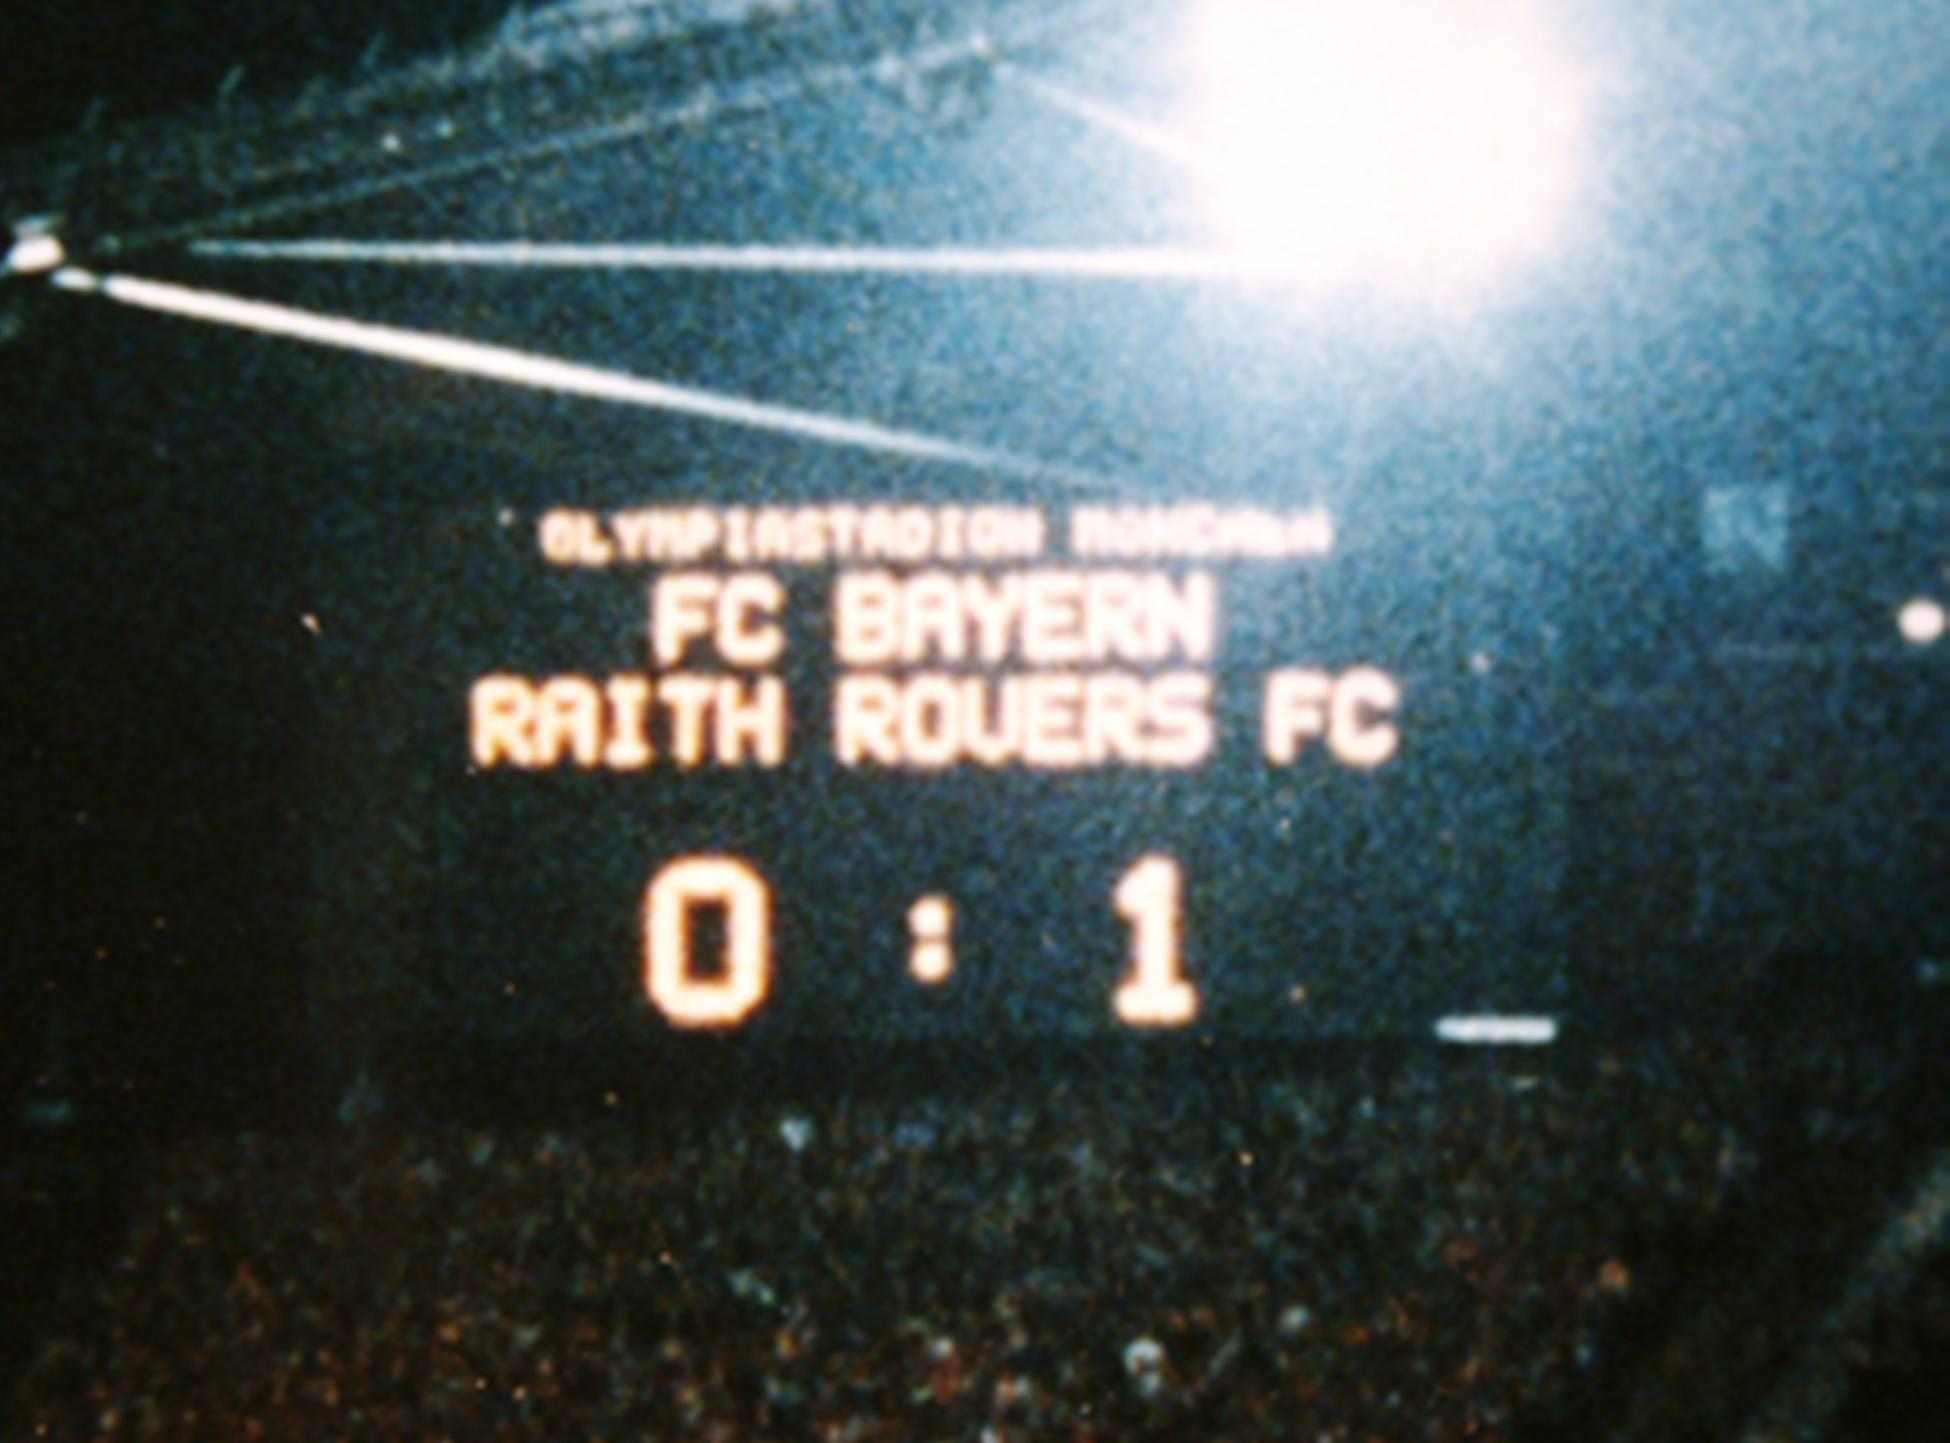
\includegraphics[width=0.65\textwidth,height=0.65\textheight]{images/raith.jpg}
\caption{A memorable scoreboard}
\end{figure}
\end{frame}

\begin{frame}{What is Utility}
\protect\hypertarget{what-is-utility-1}{}
\begin{itemize}
\tightlist
\item
  The players would prefer a 3-4 result (i.e., 3 for them, 4 for other
  player) to a 2-1 result.
\item
  So this is very much unlike soccer, even though the numbers will often
  feel a lot like soccer scores.
\end{itemize}
\end{frame}

\begin{frame}{What is Utility}
\protect\hypertarget{what-is-utility-2}{}
\begin{itemize}
\tightlist
\item
  It's not money, for two distinct reasons.
\item
  First, the players might care how much money the other players get.
\end{itemize}
\end{frame}

\begin{frame}{Utility and Altruism}
\protect\hypertarget{utility-and-altruism}{}
Consider these three situations

\begin{enumerate}
\tightlist
\item
  Billy gets \$90, Suzy gets \$100.
\item
  Billy gets \$100, Suzy gets nothing.
\item
  Billy gets \$110, Suzy gets \$100.
\end{enumerate}

How do you order these in terms of utility to Billy, from highest to
lowest?
\end{frame}

\begin{frame}{Utility and Altruism}
\protect\hypertarget{utility-and-altruism-1}{}
\begin{itemize}[<+->]
\tightlist
\item
  We don't know given just this description.
\item
  If Billy wants Suzy to get money, he might prefer option 1 to option
  2.
\item
  If Billy wants Suzy to not have money, he might prefer option 2 to
  option 3.
\end{itemize}
\end{frame}

\begin{frame}{What is Utility}
\protect\hypertarget{what-is-utility-3}{}
\begin{itemize}
\tightlist
\item
  It's not money, for two distinct reasons.
\item
  Second, getting twice as much money typically doesn't produce twice as
  much utility.
\end{itemize}
\end{frame}

\begin{frame}{What is Utility}
\protect\hypertarget{what-is-utility-4}{}
It is, more or less, desirability.

\begin{itemize}
\tightlist
\item
  Outcome \(O_1\) has more utility for player \(X\) than outcome \(O_2\)
  iff \(X\) prefers to be in \(O_1\) than \(O_2\).
\end{itemize}
\end{frame}

\begin{frame}{Utility and Numbers}
\protect\hypertarget{utility-and-numbers}{}
\begin{itemize}
\tightlist
\item
  Now you might have noticed something odd there.
\item
  We are trying to define this numerical quantity, but we've just told
  you something about when it is bigger or smaller.
\item
  Surely we need to say something more, like how much bigger or smaller
  it is in different situations.
\end{itemize}
\end{frame}

\begin{frame}{For Next Time}
\protect\hypertarget{for-next-time}{}
\begin{itemize}
\tightlist
\item
  We will start working on that very question.
\end{itemize}
\end{frame}

\end{document}
